
%% bare_conf.tex
%% V1.3
%% 2007/01/11
%% by Michael Shell

\documentclass[conference]{IEEEtran}

\usepackage{booktabs}
\usepackage{tikz}
\usepackage{url}
\usepackage{pdfpages}
\usepackage{afterpage}
\usepackage{color, colortbl}
\usepackage{graphicx} 
\usepackage{amsmath}
\usepackage{subfigure}
\usepackage{footmisc}
\usepackage{epstopdf}
\usepackage{etoolbox}
\graphicspath{{./figures/}}
%\usepackage{caption}% http://ctan.org/pkg/caption
%\captionsetup[table]{justification=centering,font={sc,small}}%


\makeatletter
%\patchcmd{\@makecaption}
%{\scshape}
%{}
%{}
%{}
%\makeatletter
\patchcmd{\@makecaption}
{\\}
{.\ }
{}
{}
\makeatother
\def\tablename{Table}

\begin{document}

\begin{figure*}[ht]
	\centering     %%% not \center
	\subfigure%%[]
	{
		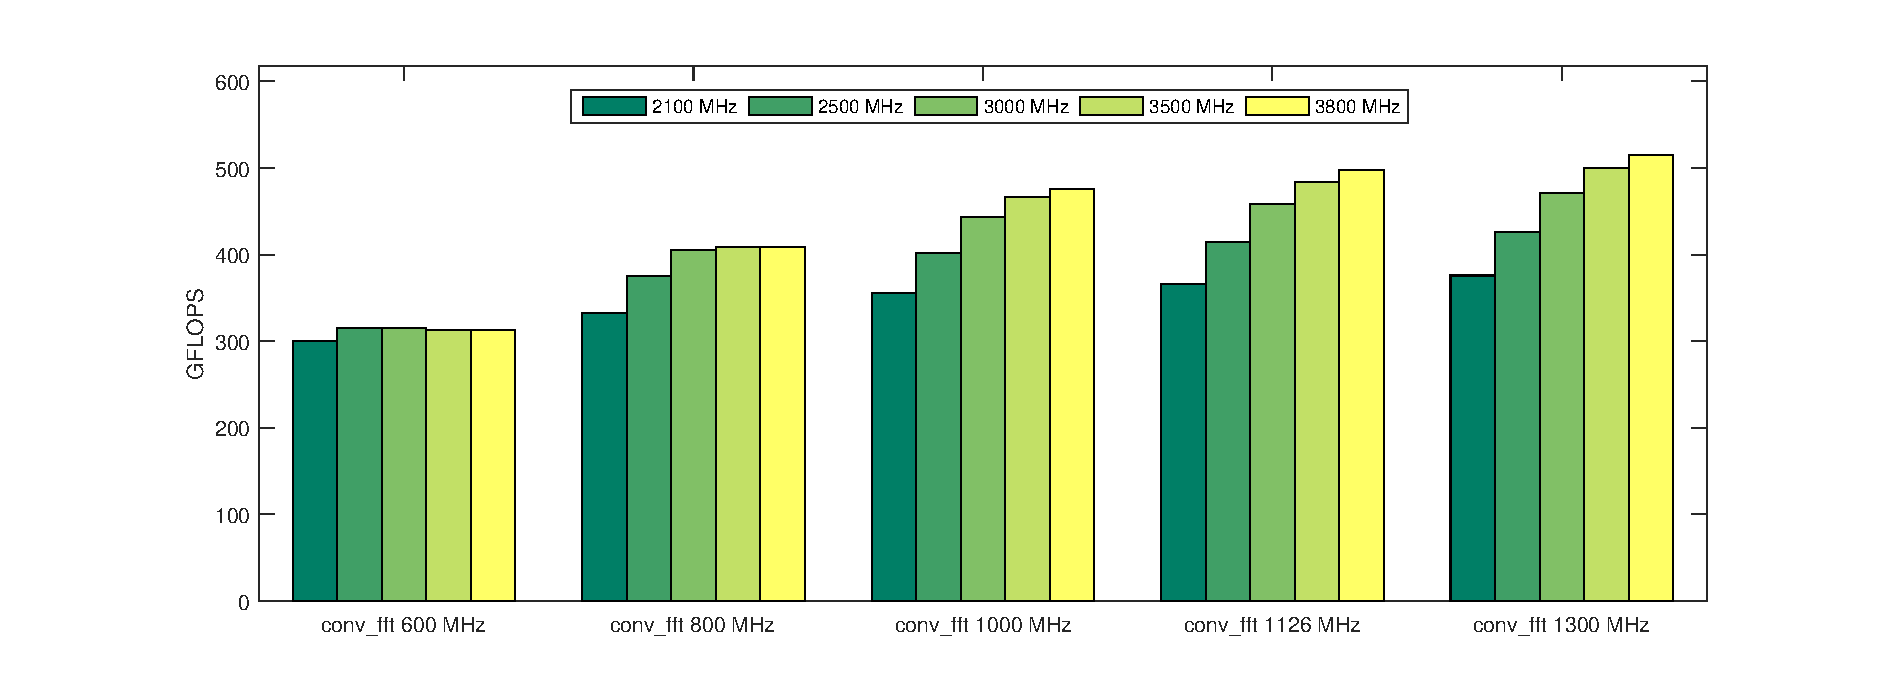
\includegraphics[width=0.9\linewidth]{perf_fft.eps}
	}
	\subfigure%%[]
	{
		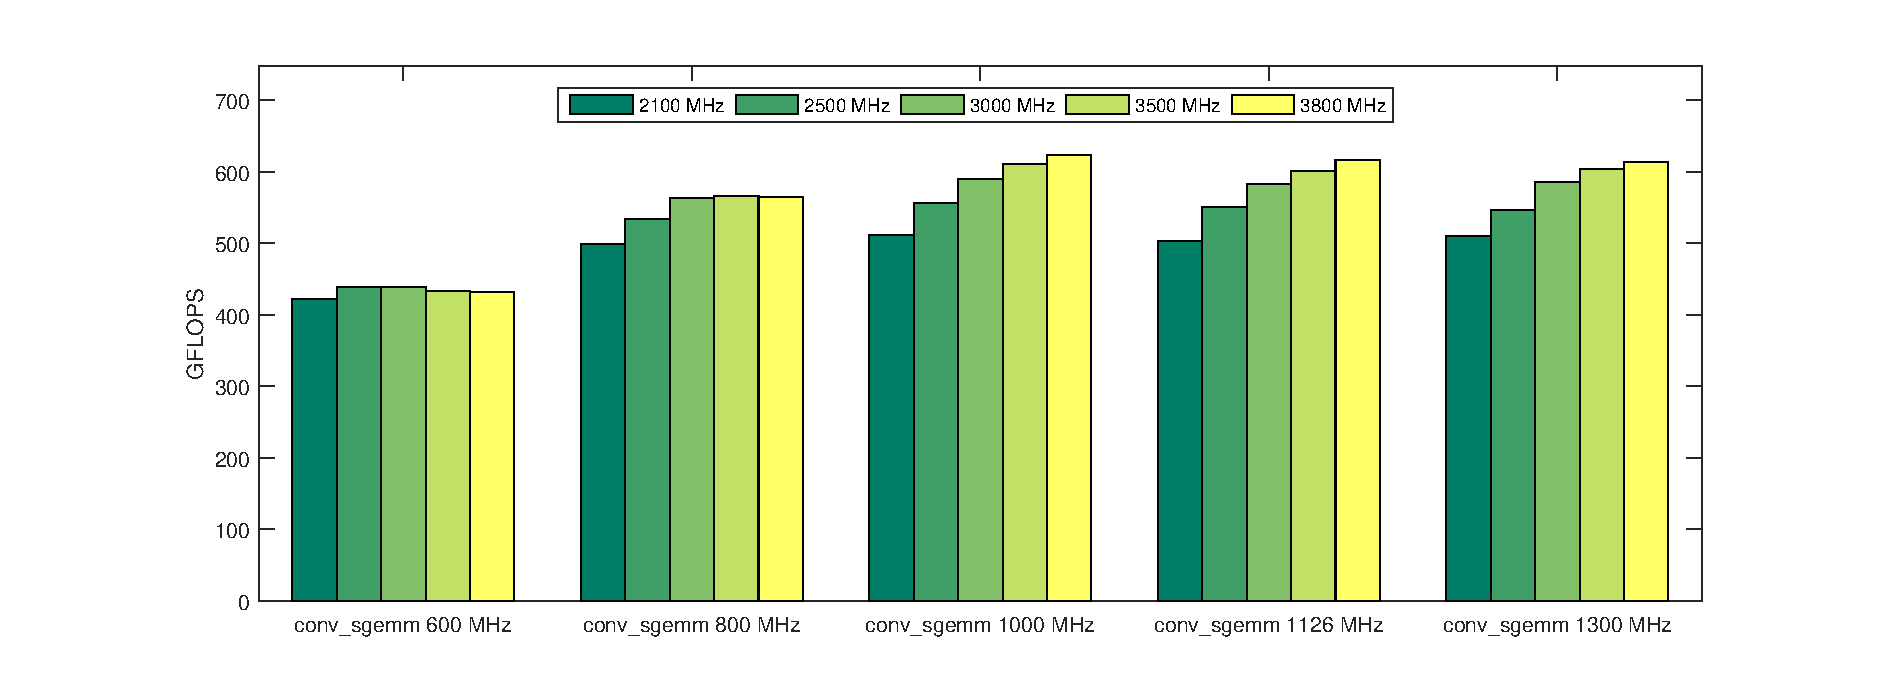
\includegraphics[width=0.9\linewidth]{perf_sgemm.eps}
	}
	\subfigure%%[]
	{
		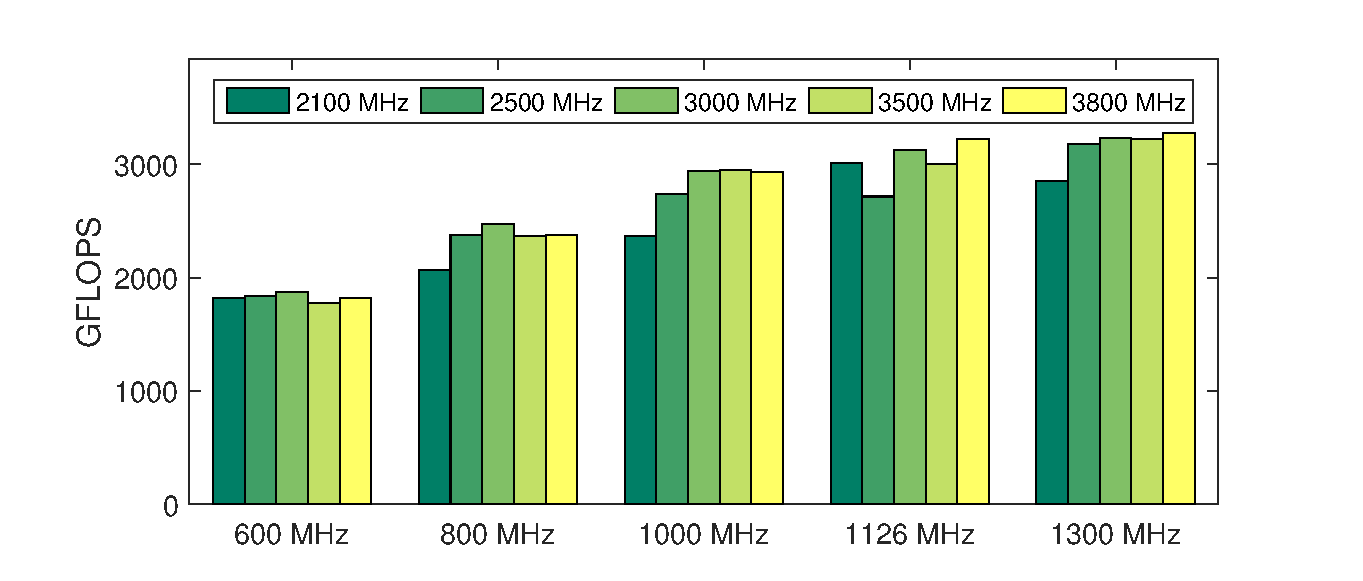
\includegraphics[width=0.9\linewidth]{perf_winograd.eps}
	}
	\caption{\label{fig:perf} Performance figures.}
\end{figure*}

\begin{figure*}[ht]
	\centering     %%% not \center
	\subfigure%%[]
	{
		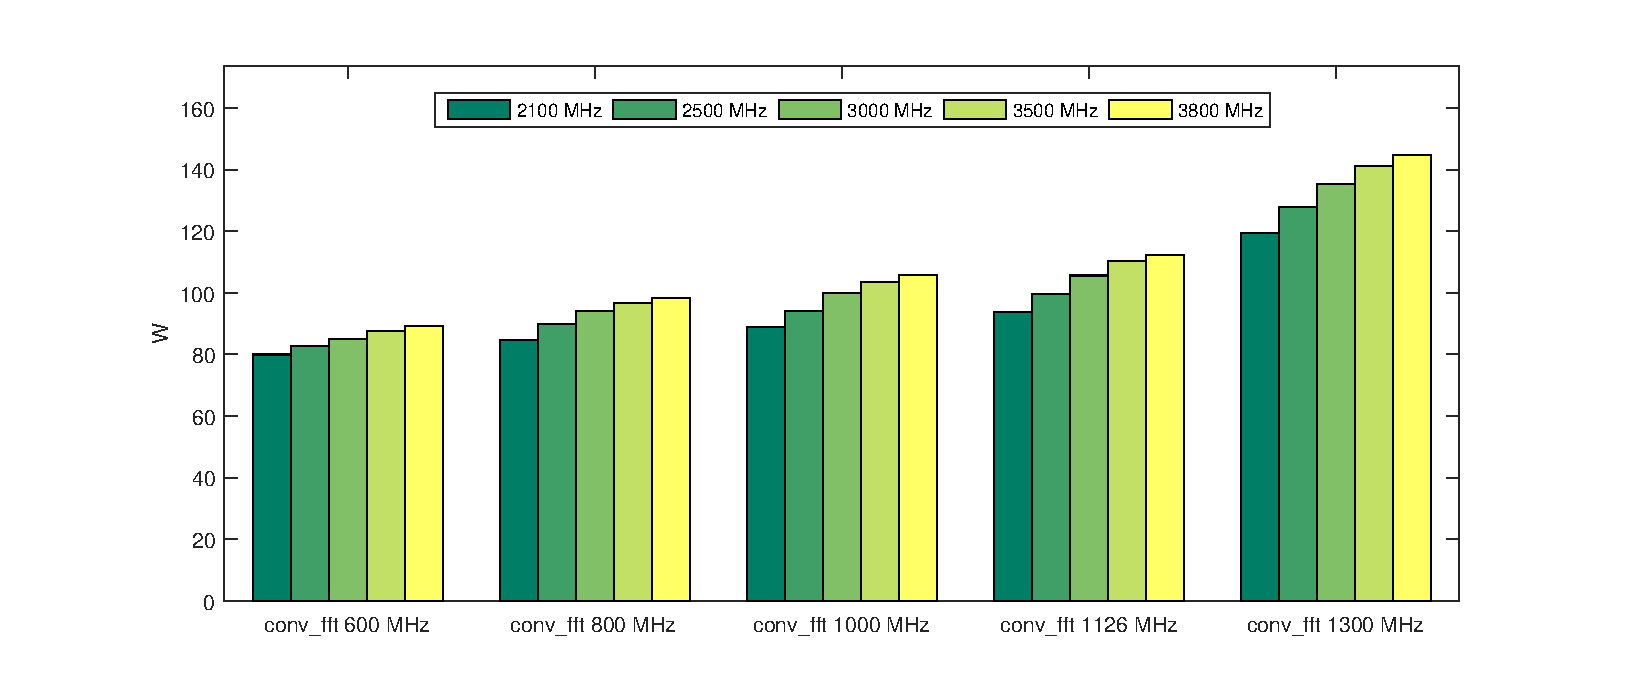
\includegraphics[width=0.9\linewidth]{power_fft.eps}
	}
	\subfigure%%[]
	{
		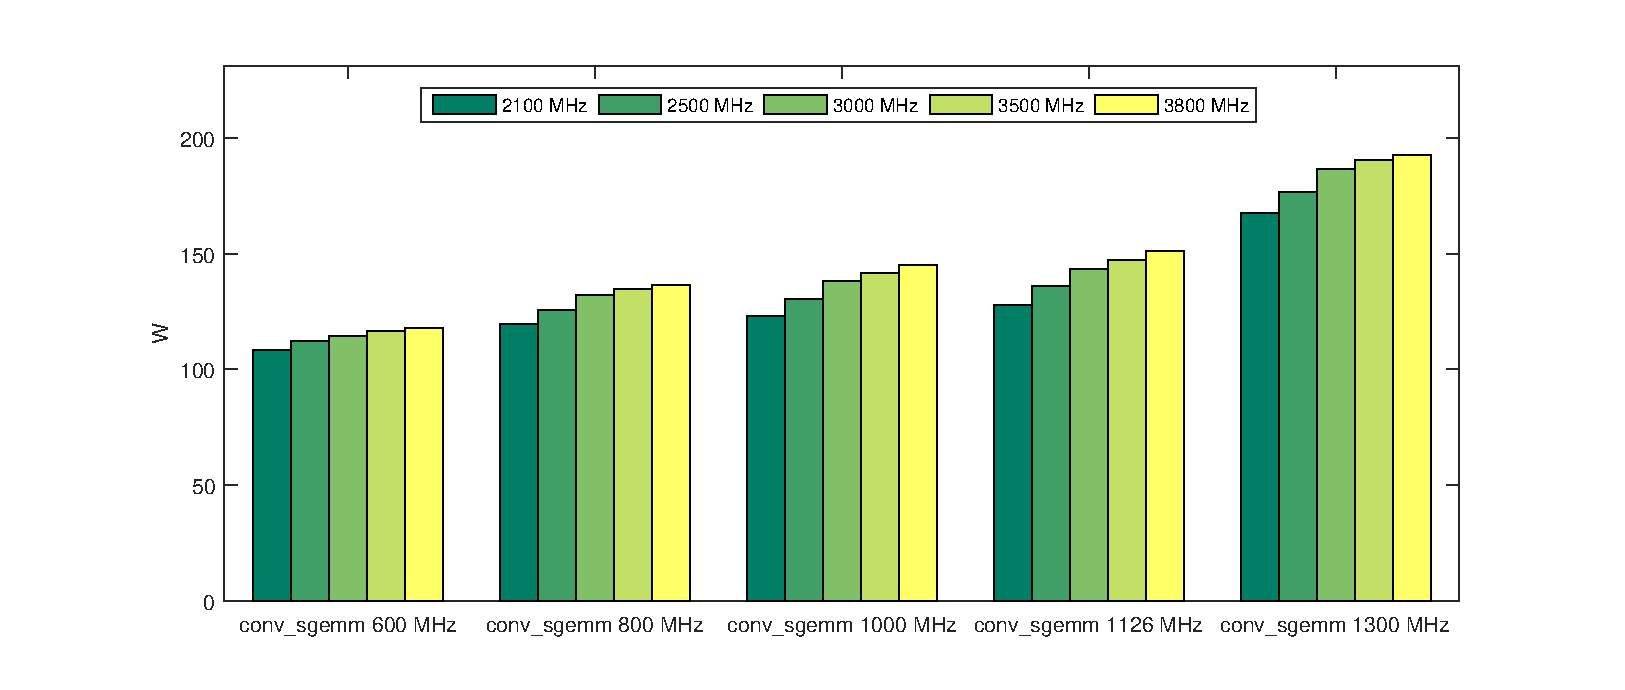
\includegraphics[width=0.9\linewidth]{power_sgemm.eps}
	}
	\subfigure%%[]
	{
		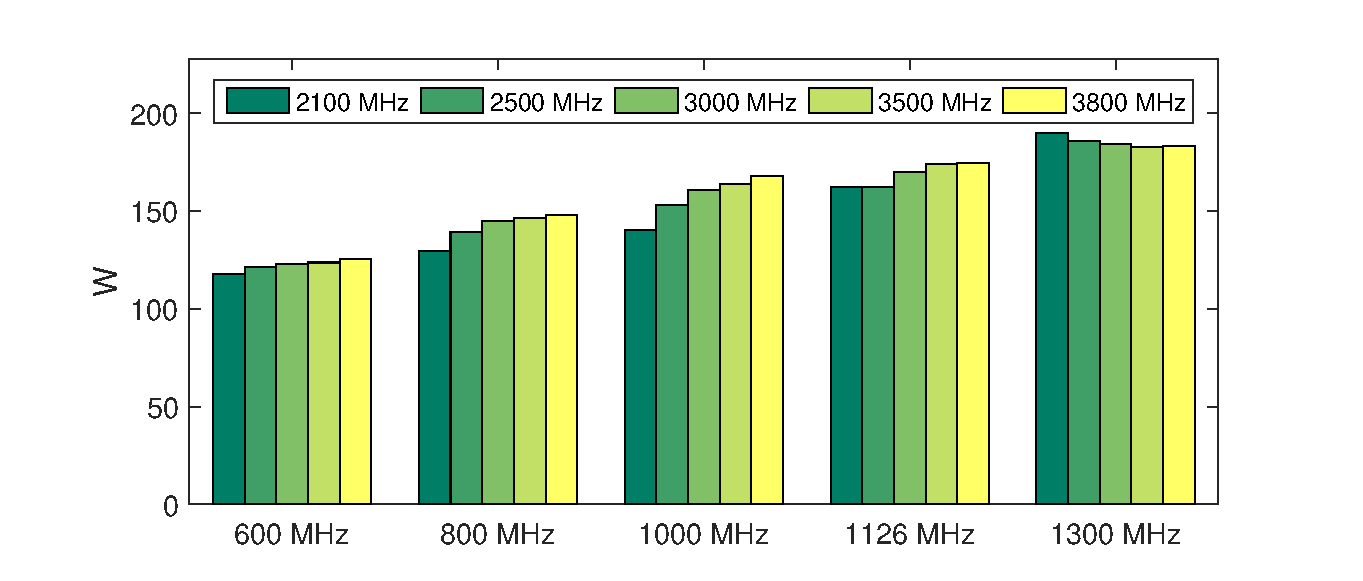
\includegraphics[width=0.9\linewidth]{power_winograd.eps}
	}
	\caption{\label{fig:power} Power figures.}
\end{figure*}	
	
\begin{figure*}[ht]
	\centering     %%% not \center
	\subfigure%%[]
	{
		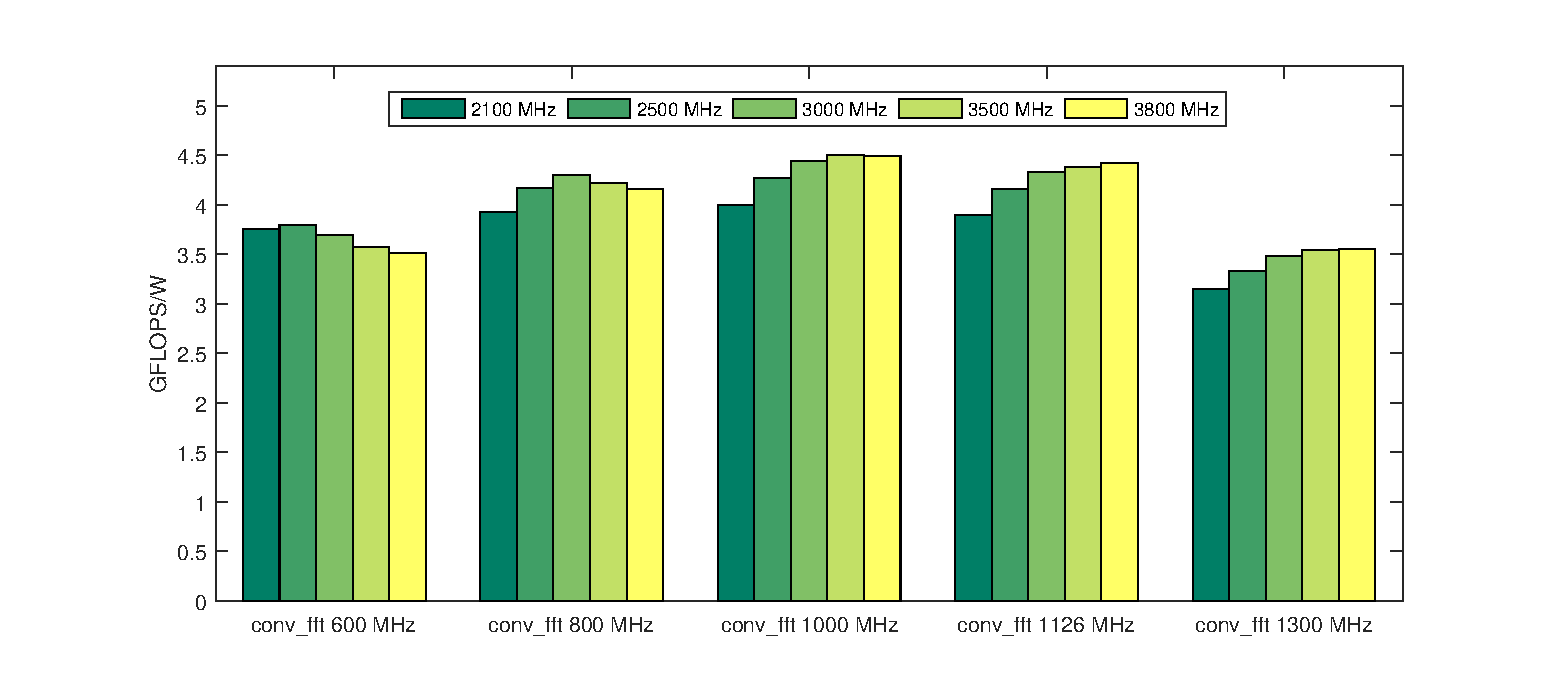
\includegraphics[width=0.9\linewidth]{ee_fft.eps}
	}
	\subfigure%%[]
	{
		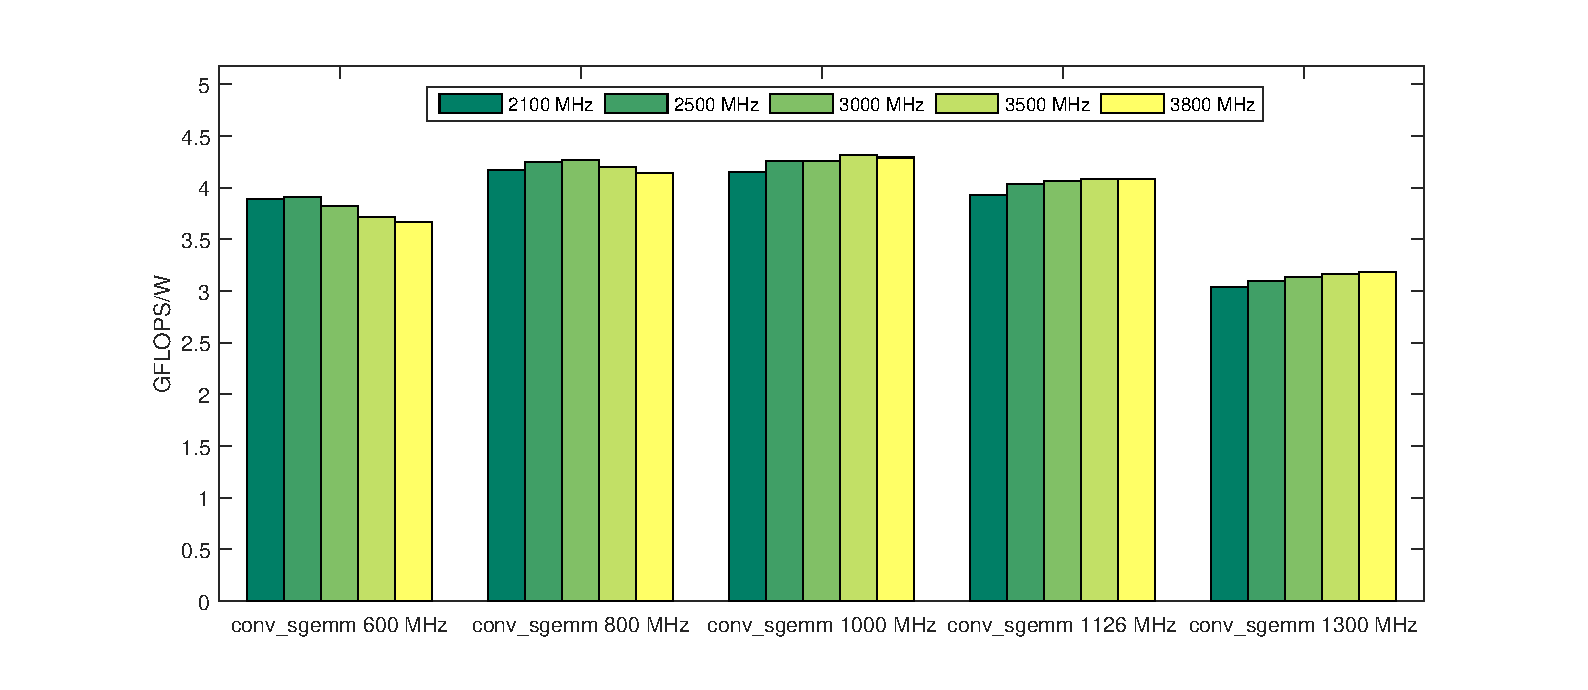
\includegraphics[width=0.9\linewidth]{ee_sgemm.eps}
	}
	\subfigure%%[]
	{
		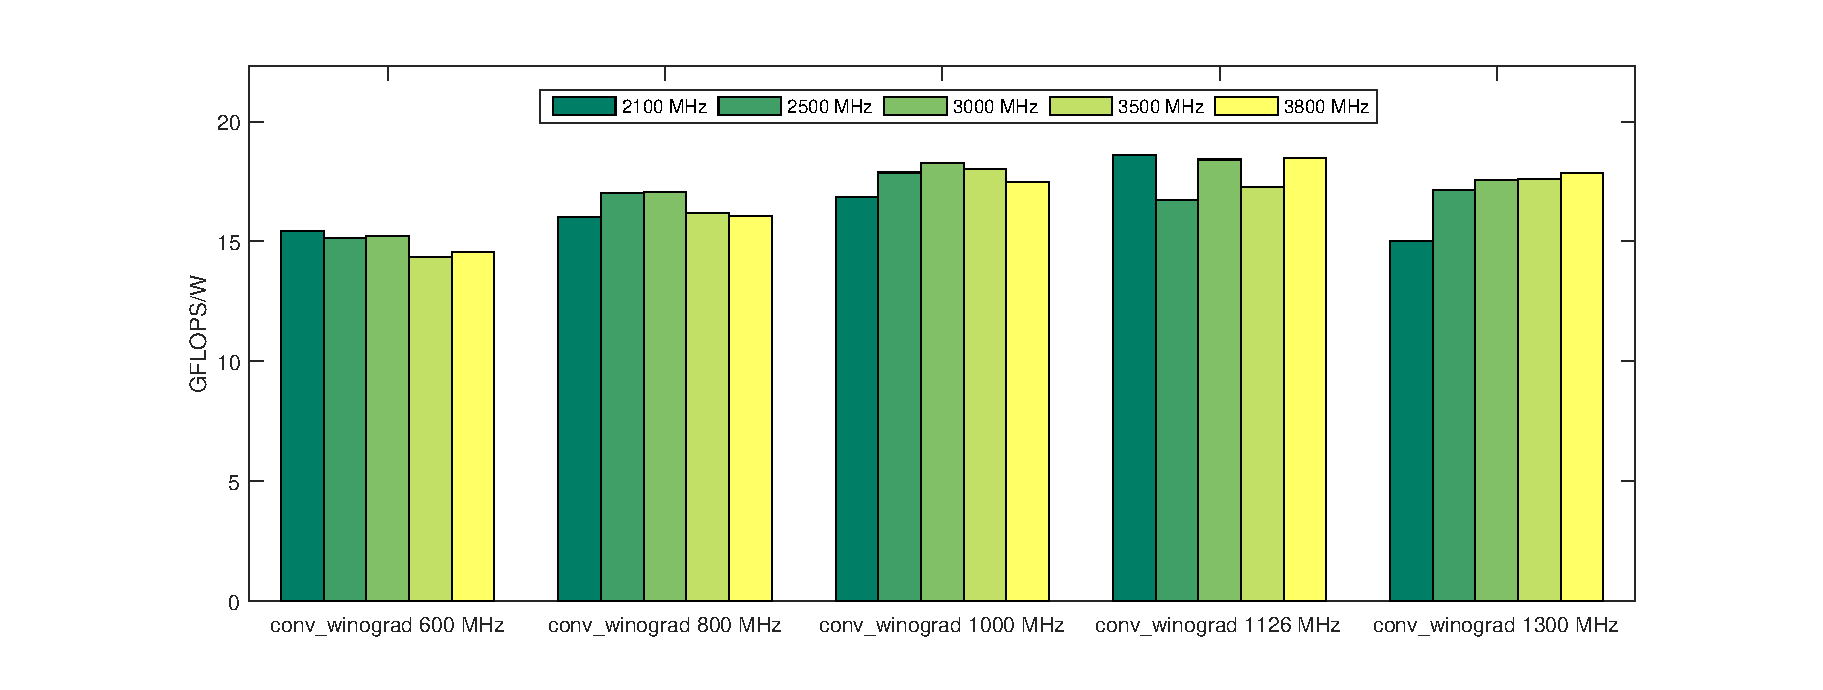
\includegraphics[width=0.9\linewidth]{ee_winograd.eps}
	}
	\caption{\label{fig:ee} Energy Efficiency figures.}
\end{figure*}



% that's all folks
\end{document}


